\section{ROSAA Numerical simulation}
\label{subsec:CD+-kinetics-simulation}

In this section, we shall discuss the results from the numerical simulation of
the ROSAA processes described in detail in Section
\ref{subsec:ROSAA-simulation}.

\subsection{Collisional process}
\label{subsec:CD+-kinetics-simulation-coll}

As the hot \CD ions from the ion source (T$_{coll}=300$ K) enter the 22-pole
ion trap (T$_{trap}=4.8(3)$ K), they are collisionally cooled down by He buffer
gas atoms and, at equilibrium, reach the effective collision temperature
(T$_{coll}=7(1)$ K). The T$_{coll}$ is derived using T$_{ion}$ and T$_{trap}$
temperature as described in Eq. \ref{eqn:Tcoll} (see Section
\ref{subsec:CD+-Tion}). In the absence of radiation and attachment processes,
the collisional process reaches an equilibrium of the relative population of
rotational quantum states, which is given by the Boltzmann distribution (at
\Tcoll), as shown in Figure
\ref{fig:ROSAA-sim-collisional-boltzman-comparision} (see Section
\ref{subsec:ROSAA-simulation-coll}). The collisional rate coefficient values
are derived from \citet{Werfelli2017}, for T$_{coll}=7$ K, the rate constants
for $J=0-5$ are given in Appendix Table
\ref{appendix:tab:collisional-rate-coefficients}. The rates are in the order of
$>10^4$ \pers\ for $2.2 \cdot 10^{14}$ \percc\ helium number density. As can be
seen in Fig. \ref{fig:ROSAA-sim-collisional-boltzman-comparision},
thermalization of the initially hot ions to the Boltzmann distribution at the
collisional temperature happens within 0.3 ms under typical experimental
conditions.

\begin{figure}[!htb]
    % \centering
    \Subfigure[0.49]{\includegraphics[width=1\textwidth]{figures/simulations/collisional/CD+_He_f-time__transition_0-1_0.001s_population_ratio.pdf}}{}{\label{fig:ROSAA-sim-collisional}}
    \hfill
    \Subfigure[0.49]{\includegraphics[width=1\textwidth]{figures/simulations/collisional/CD+_He_f-time__transition_0-1_0.001s_boltzman_comparision.pdf}}{}{\label{fig:ROSAA-sim-collisional-boltzmann}}
    
    \caption{(a) Collisional process for \CD ions up to $J=5$ with He buffer gas ([He]$=2.2 \cdot 10^{14}$ \percc). The coloured label indicates the corresponding \CD$(J)$ state. At $t=0$, T$_{coll}=300$ K, at which the relative population corresponds to a Boltzmann distribution at 300 K. The relative population evolves through collisions with He with rate constants for T$_{coll}=7$ K (derived from \cite{Werfelli2017}), subsequently reaching equilibrium after $<0.5$ ms. (b) Comparison of the Boltzmann distribution at 7 K with the relative population involving only collisional process (Coll.) at $t=1$ ms.}
    \label{fig:ROSAA-sim-collisional-boltzman-comparision}
\end{figure}
The spontaneous emission rates $(A)$ are also included in this process, as discussed in section \ref{subsec:ROSAA-simulation-spont}. However, the collision process dominates it by $8$ orders of magnitude (see Table \ref{appendix:tab:collisional-rate-coefficients} and \ref{appendix:tab:radiative-rate-coefficients}). Therefore, in the following sections, spontaneous emission rates will not be mentioned specifically, although it is included in all the cases during simulation.

\subsection{Radiative processes}
\label{subsec:CD+-kinetics-simulation-coll-rad}

As discussed above, when including only the collisional process, the relative
population re-distributed from room temperature (300 K) to Boltzmann
distribution (T$_{coll}=7$ K) at equilibrium within $<0.5$ ms. Furthermore, in
the presence of radiation resonant with $J=0-1$ of \CD, the population can be
further re-distributed due to a competing radiative process as shown in Figure
\ref{fig:ROSAA-sim-coll-rad-population-boltzmann}. The simulation of the
evolution of the relative population of the \CD$(J)$ rotational levels is shown
in Figure \ref{fig:ROSAA-sim-coll-rad-population} for a duration of 1 ms. The
derivation of radiative rates is described in detail in section
\ref{subsec:ROSAA-simulation-rad}. The radiative rates for power $35\ \mu$W are
in the same order of magnitude as collisional rates, i.e., $>10^{4}$ \pers\
(see Table \ref{appendix:tab:radiative-rate-coefficients}).

\begin{figure}[!htb]
    % \centering
    \Subfigure[0.49]{\includegraphics[width=1\textwidth]{figures/simulations/coll_rad/CD+_He_f-time__transition_0-1_0.001s_population_ratio.pdf}}{}{\label{fig:ROSAA-sim-coll-rad-population}}
    \hfill
    \Subfigure[0.49]{\includegraphics[width=1\textwidth]{figures/simulations/coll_rad/CD+_He_f-time__transition_0-1_0.001s_boltzman_comparision.pdf}}{}{\label{fig:ROSAA-sim-coll-rad-boltzmann}}
    
    \caption{(a) Simulated relative rotational level populations for \CD as labelled in parenthesis. The population evolves from $t=0$ (T$_{coll}=300$ K) to reach equilibrium at $t<0.5$ ms. The solid and dashed lineshapes correspond with (ON) and without (OFF) the presence of radiation for \CD \CDline transition. The radiation power is $35\ \mu$ W. (b) Compares the Boltzmann distribution at 7 K with the relative population involving only collisional process (Coll.) and, collision and radiative process (Coll. + Rad.) at $t=1$ ms.}
    \label{fig:ROSAA-sim-coll-rad-population-boltzmann}
\end{figure}


As depicted in Figure \ref{fig:ROSAA-sim-coll-rad-boltzmann}, the distribution
no longer follow a Boltzmann distribution. Furthermore, if the radiative rates
dominate the collisional rates (Coll. $\ll$ Rad), say for power $10^{5}$
higher, i.e., 3.5 W, we get rates in the order of $>10^{7}$ \pers. The
resulting population on $J=0$ and $J=1$ quantum levels should then reach their
statistical weights ($g(J) = 2J + 1$). The simulated relative population
evolution and equilibrium population under the condition Coll. $\ll$ Rad. is
shown in Figure \ref{fig:ROSAA-sim-coll-rad-population-boltzmann-higher-rad},
for a duration of 1 ms. And Figure
\ref{fig:ROSAA-sim-coll-rad-boltzmann-higher-rad} also clearly shows the $J=0$
and $J=1$ rotational states reaching their statistical weight of 0.25 and 0.75,
respectively.

\begin{figure}[!htb]
    % \centering
    \Subfigure[0.49]{\includegraphics[width=1\textwidth]{figures/simulations/coll_rad/CD+_He_f-time__transition_0-1_0.001s_population_ratio-higher-rad.pdf}}{}{\label{fig:ROSAA-sim-coll-rad-population-higher-rad}}
    \hfill
    \Subfigure[0.49]{\includegraphics[width=1\textwidth]{figures/simulations/coll_rad/CD+_He_f-time__transition_0-1_0.001s_boltzman_comparision-higher-rad.pdf}}{}{\label{fig:ROSAA-sim-coll-rad-boltzmann-higher-rad}}
    
    \caption{(a) Simulated relative rotational level populations for \CD and corresponding number $J$ levels as labelled in parenthesis. The population evolves from $t=0$ (T$_{coll}=300$ K) to reach equilibrium at $t<0.5$ ms. The solid and dashed lineshapes correspond with (ON) and without (OFF) the presence of radiation on the \CD \CDline transition. The radiation power is 3.5 W. (b) Compares the Boltzmann distribution at 7 K with the relative population involving only collisional process (Coll.), collision and radiative process for power $3.5\ \mu$W (Coll. + Rad.), and collision and radiative process for power 3.5 W (Coll. $\ll$ Rad.), at $t=1$ ms.}
    \label{fig:ROSAA-sim-coll-rad-population-boltzmann-higher-rad}
\end{figure}

The next section investigates the helium attachment process, vital in
understanding the ROSAA signal, i.e., the measured rotational spectrum
intensity.

\subsection{Attachment processes}
\label{subsec:CD+-kinetics-simulation-coll-rad-att}

As the \CD ion collides with the He buffer gas at low temperature and high
number density, it forms He complexes, i.e., He$_n$\CD. The formation and
subsequent dissociation rate coefficients of He$_n$\CD are discussed in section
\ref{subsec:rate-constants}. The numerical simulation method for the attachment
process is described in detail in Section \ref{subsec:ROSAA-simulation-att}.

The ROSAA action spectroscopic technique method utilises the rotation-specific
rate coefficients for the helium attachment process to observe the change in
helium-complex formed at resonant frequency (see Section
\ref{sec:methods:rotation}). Since, as discussed above, involving radiative
processes re-distributes the population of rotational quantum states. They
subsequently result in different numbers of complexes formed, thus a
ROSAA-signal, i.e., depletion counts [\%] of He\CD as shown in Figure
\ref{fig:thz:HeCD+}.

A complete simulation involving the radiation, collisional, and attachment
processes is vital to investigate the experimentally measured rotational
spectrum, i.e., ROSAA-signal intensity. However, a rotational state-specific
rate coefficient is required to include the attachment process, which is not
straightforward to measure directly. Nevertheless, as discussed in section
\ref{sec:CD+-kinetics}, the weighted rate coefficient was measured for \CD + He
kinetic reaction, with and without the presence of radiation resonant with
$J=0-1$ transition for \CD ion, and this allows to obtain the ratio between the
rate-coefficients in the two rotational levels.

Since the relative population of ${\text{CD}^+}(0) + \text{CD}^+(1) \geq 0.97 $
at T$_{coll}=7$ K (see Figure \ref{fig:ROSAA-sim-collisional}), we can assume a
2-level quantum system to determine the rotational state-specific ternary rate
constants ($k_{3_1}(J)$) from the measured, weighted ternary rate coefficients
($k_{3_1}$) using Equation \ref{eqn:rate-constant-weighted}. The $k_{3_1}$
ratio (also referred to as \qt{$a$}) is given by:

\begin{equation}
    \begin{split}
        a & = \frac{k_{3_1}(J=1)}{k_{3_1}(J=0)}\\
        & = \frac{X \cdot \text{CD}^+(0) - \text{CD}^+(0)_{on}}{\text{CD}^+(1)_{on} - X\cdot \text{CD}^+(1)}
    \end{split}
    \label{eqns:rate-constant-change-ratio}
\end{equation}

where $X$ is the ratio of measured weighted rate constant with (ON) and without
(OFF) radiation, i.e., $X=k_{3_1}(ON) / k_{3_1}(OFF)$, \CD$(0)$ and \CD$(1)$
represents \CD rotational population ratio at $J=0$ and $J=1$, respectively.
The subscript $on$ indicates the relative population in the presence of
radiation; otherwise no radiation was admitted.\\

Using $k_{3_1}(ON)$ and $k_{3_1}(OFF)$ value from equation \ref{eqn:k-on-off},
we get $X$ as:

\begin{equation}
    X = 0.76
    \label{eqn:derived-X-value}
\end{equation}

and for the following condition \footnote{\textit{refer Section
        \ref{subsec:rot:power} for power derivation, Section
        \ref{subsec:collisional-ion-temperature} and Figure \ref{eqn:Tcoll} for
        T$_{coll}$ derivation}},

\begin{align*}
    T_{coll} & = 7\ \text{K}                      \\
    [He]     & = 2.2 \cdot 10^{14}\ \text{\percc} \\
    P        & = 3.5 \cdot 10^{-5}\ \text{W}
\end{align*}

the relative population for \CD$(J)$ is given as (see Figure
\ref{fig:ROSAA-sim-collisional} and \ref{fig:ROSAA-sim-coll-rad-population}):

\begin{align}
    \cd^+(0)      & = 0.9                                  \\
    \cd^+(1)      & = 0.1                                  \\
    \cd^+(0)_{on} & = 0.4                                  \\
    \cd^+(1)_{on} & = 0.6 \label{eqn:CD+-population-value}
\end{align}

Substituting equations \ref{eqn:derived-X-value} through
\ref{eqn:CD+-population-value} in Eq. \ref{eqns:rate-constant-change-ratio}, we
can get experimentally derived $k_{3_1}$ ratio as:

\begin{equation}
    a = 0.5
    \label{eqn:k31-ratio}
\end{equation}

The derived $k_{3_1}$ ratio value, $a=0.5$, agrees well with the previously
estimated value $a=0.55(5)$ from \citet{Brunken2017}. In the previous study,
\cite{Brunken2017}, the \qt{$a$} value is estimated by measuring \CDline
transition of \CD at different number density and radiation power and fitting
the measured ROSAA depletion signal intensity to the numerical model. However,
in this study, the \qt{$a$} is experimentally derived from kinetic measurement
in the presence and absence of radiation resonant with \CDline of \CD molecular
ion. This approach also directly validates the equation
\ref{eqn:rate-constant-weighted}, thereby, the rotational state-dependent
attachment of rare gas atoms to molecular ions. In addition, this
systematically supports our investigation of various processes involved in the
ROSAA technique. And as described in Section \ref{sec:CD+-kinetics-motivation},
the main motivation is to develop a robust general-purpose ROSSA numerical
model and be adaptable to systematically add various processes.

In the following section, the derived \qt{$a$} is used to analyse the full
model, including collisional, radiation and attachment process to the measured
pure rotational transition intensity of \CD ion.

\subsection{Analysing numerical results}
\label{subsec:CD+-kinetics-simulation-analysis}

The full model simulation, i.e., including collisional, radiation and
attachment process for \CD molecular ion up to 5 rotational quantum states
($J=0-5$), is shown in Figure \ref{fig:thz-sim:rel-pop:1ms} for 7 K
temperature, $2.2 \cdot 10^{14}$ \percc\ helium number density, $k_{3_1}$
ratio, $a=0.5$ and $3.5\ \mu$W power.
% In addition to \CD, the simulation considers up to two complexes (He\CD and He$_2$\CD) at 7 K temperature, $2.2 \cdot 10^{14}$ \percc\ helium number density, $k_{3_1}$ ratio, $a=0.5$ and $3.5\ \mu$W power. 
The \CD$(J)$ ion for $J>3$ becomes insignificant within $<0.5$ ms, i.e.,
reaches $\ll 10^{-10}$ in relative population ratio while \CD(2) and \CD(3)
equilibrates to $<10^{-2}$ and $<10^{-6}$, respectively in relative population
ratio. Therefore, in this simulation under 2-level system assumption, the
ternary attachment rate coefficients $k_{3_1}(J\geq 2)=0$, i.e., only the
\CD$(J=0)$ and \CD$(J=1)$ participates in the cluster formation. However, the
\CD$(J \geq 2)$ is included in the simulation to monitor its relative
population evolution.

% \begin{figure}
    \centering
    \includegraphics[width=1\textwidth]{figures/simulations/coll_rad_att/CD+_He_f-time__transition_0-1_0.001s_population_ratio.pdf}
    \caption{Simulated relative rotational level populations for \CD and corresponding number He$_n$\CD clusters (n=1, 2) as labelled in (top right) and \CD$(J)$ indicates \CD in $J$ rotational state. The simulation conditions are as follows: $k_{3_1}$ ratio, $a=0.5$, collisional rates for T$_{coll}=7$ K  (at $t=0$, T$_{coll}=300$ K), Helium number density $2.2 \cdot 10^{14}$ \percc and radiation power $3.5\cdot10^{-5}$ W. The solid and dashed lines correspond to, with (-ON) and without (--OFF), the presence of radiation for \CD \CDline transition.}
    \label{fig:thz-sim:rel-pop:1ms}
\end{figure}
\begin{figure}[!htb]
    \centering
    \begin{adjustbox}{minipage=\linewidth,scale=0.7}
    \Subfigure[0.8]{\includegraphics[width=1\textwidth]{figures/simulations/coll_rad_att/CD+_He_f-time__transition_0-1_0.001s_population_ratio.pdf}}{}{\label{fig:thz-sim:rel-pop:1ms}}
    \hfill
    
    \Subfigure[0.5]{\includegraphics[width=1\textwidth]{figures/simulations/coll_rad_att/CD+_He_f-time__transition_0-1_0.6s_population_ratio.pdf}}{}{\label{fig:thz-sim:rel-pop:0.6s}}
    \hfill
    \Subfigure[0.45]{\includegraphics[width=1\textwidth]{figures/simulations/coll_rad_att/CD+_He_f-time__transition_0-1_0.6s_signal.pdf}}{}{\label{fig:thz-sim:signal:0.6s}}
    \hfill
    
    \Subfigure[0.5]{\includegraphics[width=1\textwidth]{figures/simulations/coll_rad_att/CD+_He_f-time__transition_0-1_100.0s_population_ratio.pdf}}{}{\label{fig:thz-sim:rel-pop:100s}}
    \hfill
    \Subfigure[0.45]{\includegraphics[width=1\textwidth]{figures/simulations/coll_rad_att/CD+_He_f-time__transition_0-1_100.0s_signal.pdf}}{}{\label{fig:thz-sim:signal:100s}}
    \hfill
    
    \end{adjustbox}
    
    \caption{(a) Simulated relative rotational level populations for \CD and corresponding numberof He$_n$\CD clusters (n=1, 2) where \CD$(J)$ indicates \CD in $J$ rotational state. The simulation conditions are as follows: $k_{3_1}$ ratio, $a=0.5$, collisional rates for T$_{coll}=7$ K  (at $t=0$, T$_{coll}=300$ K), Helium number density $2.2 \cdot 10^{14}$ \percc and radiation power $3.5\cdot10^{-5}$ W. The solid and dashed lines correspond to, with (-ON) and without (--OFF), the presence of radiation on the \CD \CDline transition frequency. The simulation duration for (a) 1 ms, (b) 600 ms and (d) 100 s. Figures (c) and (e) correspond to signal intensity, i.e., He\CD depletion \% as a function of time for (b) and (d), respectively.}
    
    \label{fig:thz-sim:rel-pop}

\end{figure}


The attachment and dissociation rates timescale are in the order of $10^{-1}$
\pers\ (see Table \ref{appendix:tab:attachment-rate-coefficients}). Thus, the
first complex (He\CD) population is very small, i.e., $<10^{-4}$ in relative
population, during the first 1 ms; however, it tends to increase. Therefore,
when the simulation is extended for a longer duration, i.e., for 600 ms (see
Figure \ref{fig:thz-sim:rel-pop:0.6s}) and 100 s (see Figure
\ref{fig:thz-sim:rel-pop:100s}), the He\CD relative population reaches 0.03 and
attains equilibrium at 0.2 after 40 s, respectively. Also, as our initial
consideration of a 2-level quantum system, the former and latter figures
supports this assumption, i.e., at 7 K temperature and $t=0.6$ s duration, 
the relative population pumped into \CD(0)$=0.86$ and \CD(1)$=0.11$ 
but for \CD$(J\geq 2)$ is $\ll 10^{-4}$.

As expected, and shown in Figure \ref{fig:thz-sim:rel-pop:0.6s} and
\ref{fig:thz-sim:rel-pop:100s}, a significant difference in population is
observed in the first He\CD complex with (-ON) and without (-\--OFF) the
presence of radiation resonant with the \CDline transition of \CD. This
difference is indeed the measured ROSAA depletion signal of He\CD at resonance.
Figure \ref{fig:thz-sim:signal:0.6s} represent the expected signal intensity of
the measured rotational spectrum (as shown in Figure \ref{fig:thz}) for a trap
duration of 600 ms. Before analysing further, let us look at approaches to
validate our model.\\

% \begin{figure}[!htb]
    \centering
    \begin{adjustbox}{minipage=\linewidth,scale=0.7}
    \Subfigure[0.8]{\includegraphics[width=1\textwidth]{figures/simulations/coll_rad_att/CD+_He_f-time__transition_0-1_0.001s_population_ratio.pdf}}{}{\label{fig:thz-sim:rel-pop:1ms}}
    \hfill
    
    \Subfigure[0.5]{\includegraphics[width=1\textwidth]{figures/simulations/coll_rad_att/CD+_He_f-time__transition_0-1_0.6s_population_ratio.pdf}}{}{\label{fig:thz-sim:rel-pop:0.6s}}
    \hfill
    \Subfigure[0.45]{\includegraphics[width=1\textwidth]{figures/simulations/coll_rad_att/CD+_He_f-time__transition_0-1_0.6s_signal.pdf}}{}{\label{fig:thz-sim:signal:0.6s}}
    \hfill
    
    \Subfigure[0.5]{\includegraphics[width=1\textwidth]{figures/simulations/coll_rad_att/CD+_He_f-time__transition_0-1_100.0s_population_ratio.pdf}}{}{\label{fig:thz-sim:rel-pop:100s}}
    \hfill
    \Subfigure[0.45]{\includegraphics[width=1\textwidth]{figures/simulations/coll_rad_att/CD+_He_f-time__transition_0-1_100.0s_signal.pdf}}{}{\label{fig:thz-sim:signal:100s}}
    \hfill
    
    \end{adjustbox}
    
    \caption{(a) Simulated relative rotational level populations for \CD and corresponding numberof He$_n$\CD clusters (n=1, 2) where \CD$(J)$ indicates \CD in $J$ rotational state. The simulation conditions are as follows: $k_{3_1}$ ratio, $a=0.5$, collisional rates for T$_{coll}=7$ K  (at $t=0$, T$_{coll}=300$ K), Helium number density $2.2 \cdot 10^{14}$ \percc and radiation power $3.5\cdot10^{-5}$ W. The solid and dashed lines correspond to, with (-ON) and without (--OFF), the presence of radiation on the \CD \CDline transition frequency. The simulation duration for (a) 1 ms, (b) 600 ms and (d) 100 s. Figures (c) and (e) correspond to signal intensity, i.e., He\CD depletion \% as a function of time for (b) and (d), respectively.}
    
    \label{fig:thz-sim:rel-pop}

\end{figure}


% \textbf{Verifying model:}\\
% \label{subsec:CD+-kinetics-simulation-verification}

There are three direct ways to verify the validity of the numerical model.

\begin{enumerate}
    \item  One is to compare it with the Boltzmann distribution when only collisional
          processes are considered. Then at equilibrium, the relative population of
          \CD$(J)$ reaches T$_{coll}$ temperature, which should be equivalent to the
          Boltzmann distribution at T$_{coll}$. This has been discussed in Section
          \ref{subsec:CD+-kinetics-simulation-coll} and can be verified in Figure
          \ref{fig:ROSAA-sim-collisional-boltzmann}.
    \item The other way is when collisional and radiative processes are involved,
          competing with each other. Under conditions when the radiative process (for
          \CDline transition of \CD) dominates the collisional process (Coll. $\ll$
          Rad.), the equilibrium relative population of \CD$(J=0)$ and \CD$(J=1)$ should
          reach its statistical weight ($g(J) = 2J+1$), i.e., 0.25 and 0.75,
          respectively. This has been discussed in section
          \ref{subsec:CD+-kinetics-simulation-coll-rad} and can be verified in Figure
          \ref{fig:ROSAA-sim-coll-rad-boltzmann-higher-rad}.
    \item Another direct approach is to verify the signal intensity is $\sim 0$ when
          $k_{3_1}$ ratio $a=1$. This indicates that the rate constants are not
          state-dependent but rather the same, thus leading to the absence of ROSAA
          signal intensity.
\end{enumerate}

In addition to validating the third point (3) for the numerical model, similar
to the signal intensity plot as shown in Figure \ref{fig:thz-sim:signal:0.6s}
and \ref{fig:thz-sim:signal:100s}, a complete overview of signal intensity
simulations as a function of power ranging from $10^{-7}-10^{-2}$ W, number
density from $10^{12}-10^{16}$ \percc and $k_{3_1}$ ratio, $a$ ranging from
$0.3-1$, is shown in Figure \ref{fig:thz:all-simulation}. The third point can
be verified as shown in Figure \ref{fig:thz:all-simulation:0.1a}, where the
signal intensity is 0 as expected when $a=1$.\\

\begin{figure}[!htb]
    \centering
    
    \Subfigure[0.3]{\includegraphics[width=1\textwidth]{figures/simulations/ROSAA/f-power_1e-7-1e-2/k3_branch_0.30.pdf}}{$k_{3_1}$ ratio $=0.3$}{}
    \hfill
    \Subfigure[0.3]{\includegraphics[width=1\textwidth]{figures/simulations/ROSAA/f-power_1e-7-1e-2/k3_branch_0.40.pdf}}{$k_{3_1}$ ratio $=0.4$}{}
    \hfill
    \Subfigure[0.3]{\includegraphics[width=1\textwidth]{figures/simulations/ROSAA/f-power_1e-7-1e-2/k3_branch_0.50.pdf}}{$k_{3_1}$ ratio $=0.5$}{\label{fig:thz:all-simulation:0.5a}}
    \hfill
    \Subfigure[0.3]{\includegraphics[width=1\textwidth]{figures/simulations/ROSAA/f-power_1e-7-1e-2/k3_branch_0.60.pdf}}{$k_{3_1}$ ratio $=0.6$}{}
    \hfill
    \Subfigure[0.3]{\includegraphics[width=1\textwidth]{figures/simulations/ROSAA/f-power_1e-7-1e-2/k3_branch_1.00.pdf}}{$k_{3_1}$ ratio $=1$}{\label{fig:thz:all-simulation:0.1a}}
    \hfill
    \Subfigure[0.3]{\includegraphics[width=1\textwidth]{figures/simulations/ROSAA/f-power_1e-7-1e-2/combined.pdf}}{combined}{}
    
    \caption{Numerical simulation of ROSAA process with computed signal intensities as a function of radiation power, $10^{-7} - 10^{-2}$ W, He number density, $10^{12} - 10^{16}$ \percc, and function of $k_{3_1}$ ratio, $0.3-1$, at 600 ms trap duration and T$_{coll}=7(1)$ K temperature. The captions of subplots (a)-(e) indicate the respective $k_{3_1}$ ratio value. (f) as captioned, shows the combined plots of (a)-(e).}
    \label{fig:thz:all-simulation}
\end{figure}

% \textbf{Comparing to ROSAA experiment:}\\
Experimental ROSAA signal strength under the condition of $2.2 \cdot 10^{14}$
\percc\ helium number density and $35\ \mu$W power at 600 ms trap time, is
$26(1)$\% (see Table \ref{tab:CD+_He}). With the same condition, Figure
\ref{fig:thz-sim:signal:0.6s} shows the signal intensity of 27\% at $t=600$ ms.
Therefore, there is close agreement with our numerical model simulation
results. Figure \ref{fig:thz:all-simulation:0.5a} depicts an overview of the
achievable signal intensity as a function of number density and power for $a=5$
and 600 ms duration. They are directly proportional to radiation power and are
inversely proportional to number density. We have utilised our THz radiation
source to full power without attenuation (see Section
\ref{subsec:ir:radiation-source}), with the number density adjusted for optimal
$700-1000$ counts of He\CD complexes formed for spectroscopy measurement (see
Figure \ref{fig:masspec}). As shown in Table \ref{tab:CD+_He}, we have measured
at different number densities, and $2.2 \cdot 10^{14}$ \percc\ at
T$_{trap}=$4.8(3) K (T$_{coll}=$7(1) K) appears to be an optimal condition to
achieve a signal of $27(1) \%$ which is not far from the maximum achievable
signal, i.e., $\approx 33 \%$ as shown in Figure
\ref{fig:thz:all-simulation:0.5a}.

The Ne-ROSAA measurement is shown in Figure \ref{fig:thz:NeCD+} and Table
\ref{tab:CD+_Ne}. Since pure Ne kinetics measurement was very challenging at
low temperatures due to freeze-out , it will be explored in detail in future
studies, and here we assume the same attachment and dissociation rate
coefficients as for helium. We run simulations under the following condition:

\begin{align*}
    [Ne]            & = 1.5 \cdot 10^{14} \text{ cm}^{-3} \\
    P               & = 35\ \mu \text{W}                  \\
    t               & = 600 \text{ ms}                    \\
    \text{T}_{trap} & = 8.7 \text{ K}                     \\
    \text{T}_{coll} & = 18.2 \text{ K}                    \\
\end{align*}

The experimentally measured Ne-ROSAA signal $24(1) \%$ best fits with the
simulation result ($24 \%$) but with the reduced $a=0.25$ rather than $a=0.5$,
at T$_{coll}=18.2$ K. As also discussed in \citet{Brunken2017}, $k_{3_1}(J=1)$
likely shows a steeper decreasing temperature dependence than $k_{3_1}(j=0)$.\\

Nevertheless, our initial goal was to develop an adaptable and robust numerical
simulation model (with an easy-to-use graphical user interface). In addition to
investigating He-\CD and Ne-\CD ROSAA model, it is extended to investigate the
CO$^+$ molecular ion (Chapter \ref{chapter:CO+}), which is an open-shell
species hence the rotational quantum states split intro fine structure levels
due to non-zero net electron spin. Therefore, we have shown that extending this
model to different systems is possible and will be used to predict the ROSAA
signal intensity for rotational transition measurements when given energy level
information (from the calculation) and rate coefficients from kinetic
measurements.

The next section briefly discusses an interesting observation on the
temperature dependence of ternary attachment rate coefficients.

% \clearpage